\section{Beschleunigungsräder}
    Die Vortriebskraft für die Tennisbälle wird durch zwei Beschleunigungsräder ermöglicht. Der verwendete
    Beschleunigungsradantrieb wurde aus mehreren Gründen gewählt. Über die Drehzahl und den 
    Anpressdruck der Räder kann die Wurfweite stufenlos eingestellt werden. Somit ist die Maschine 
    für jeden Tennisball in einem bestimmten Bereich gewappnet. Die Beschleunigungsräder wurden 
    aus PVC hergestellt, da dieser Werkstoff einfach zu bearbeiten ist und zugleich eine genügend 
    grosse Festigkeit bietet. Um möglichst viel Gewicht zu sparen, wurde an beiden Planflächen so 
    viel Material wie möglich herausgenommen. Für die Übertragung des Momentes auf die Welle wurde 
    ein Presssitz realisiert. Dies ermöglicht eine gleichmässige Flächenpressung und erhöht die 
    Rundlaufgenauigkeit gegenüber einer geklebten Welle-Nabe-Verbindung. Weiter ist durch die konkave Form der 
    Beschleunigungsräder die Richtung der Ballflugbahn vorgegeben. Hier wird keine zusätzliche Ballführung 
    gebraucht was Gewicht, Kosten und Platz spart. Die Räder sind konkav ausgearbeitet, so dass die 
    Beschleunigung nicht nur über einen Punkt übertragen wird. So wird gewährleistet, dass die Kraft 
    über eine grössere Fläche übertragen werden kann. Dadurch entsteht der Vorteil, dass die 
    Beschleunigung geführt abläuft, wodurch ein gerichteter Wurf entsteht. So kann die vorhandene 
    Rotationsenergie vollumfänglich den Tennisbällen übergeben werden. Die Ausrundung wird durch 
    den Radius der Bälle gegeben. Der Durchmesser der Beschleunigungsräder ist so festgelegt, dass 
    mit der vorhandenen Masse ein genügendes Trägheitsmoment zur Verfügung steht. Dies ist nötig, 
    damit bei der Beschleunigung der Tennisbälle die Räder nicht zu stark abgebremst werden. Durch 
    den Durchmesser wird auch die Winkelgeschwindigkeit festgelegt. Zudem sind die Räder mit einer 
    speziellen Haftmatte beschichtet, damit die 
    Kraft optimal auf den Ball übertragen werden kann. Somit wird ein höherer Haftreibungskoeffizient 
    erreicht und Schlupf zwischen Bällen und Beschleunigungsräder verhindert. Die Achsen der zwei Beschleunigungsräder sind im 
    Winkel von 45\si{\degree} zur Bodenplatte angeordnet. Der Abschusswinkel ist so gewählt, dass 
    die Tennisbälle mit einem genügend grossen Einschlagwinkel im Zielbereich landen. So wird die 
    Möglichkeit einer Kollision mit dem Korbrand vermieden.
    \begin{figure}[h!]
       	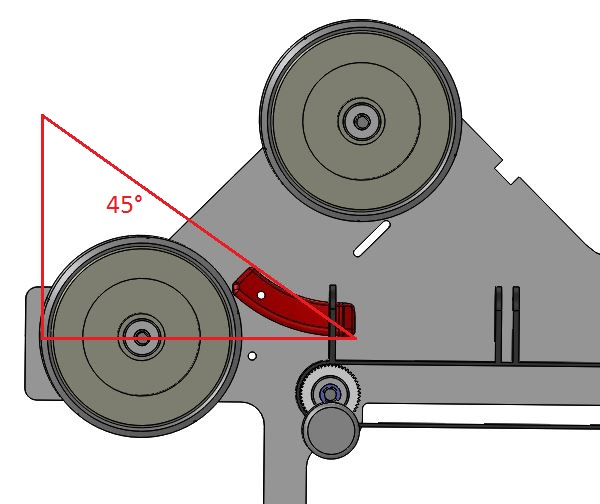
\includegraphics[width=0.5\textwidth,clip,trim=20mm 5mm 0mm 5mm]
       	{Enddokumentation/Bilder/Abschuss.JPG}
       	\centering
       	\caption{Ballzuführung mit Abschusswinkel}
       	\label{abb:Abschusswinkel}
    \end{figure}
    %    
    \subsection{Antriebsstrang}
        Für die Übertragung der Momente der Brushlessmotoren auf die Beschleunigungsräder wurde eine 
        Zahnradübersetzung von $1:4$ gewählt.
		\begin{figure}[h!]
			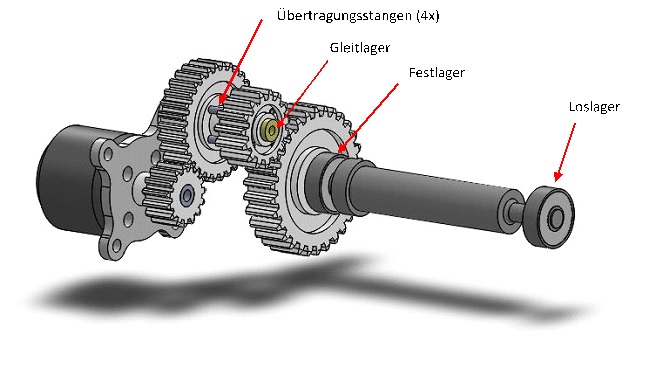
\includegraphics[width=0.9\textwidth,clip,trim=0mm 15mm 0mm 0mm]
			{Enddokumentation/Bilder/Antriebsstrang.JPG}
			\centering
			\caption{Der Antriebsstrang}
			\label{abb:Antriebsstrang}
		\end{figure}
        \begin{table}[h!]
            \centering
            \begin{zebratabular}{p{0.10\textwidth}p{0.25\textwidth}}
                \rowcolor{gray} Anzahl & Beschreibung\\
                \rule{0pt}{11pt}2x & Brushlessmotor \\
                \rule{0pt}{11pt}2x & Zahnrad Modul 1.0 Z15\\
                \rule{0pt}{11pt}2x & Zahnrad Modul 1.0 Z30\\
                \rule{0pt}{11pt}2x & Zahnrad Modul 1.25 Z15\\
                \rule{0pt}{11pt}2x & Zahnrad Modul 1.25 Z30\\
            \end{zebratabular}
            \caption{Zahnräder der Übersetzung}
            \label{tab:AntriebsstrangKraft}
        \end{table}
        Auf die Welle des Brushlessmotores wurde eine Büchse eingepresst, da die Standardbohrung des 
        Zahnrades grösser als das des Wellendurchmessers war. Das Zahnrad selber wurde ebenfalls auf die 
        Büchse aufgepresst und noch zusätzlich mit einer Stellschraube fixiert. Das grosse Zahnrad, 
        der Welle der Beschleunigungsräder, wurde ebenfalls nach dem gleichen Schema 
        montiert. Auch hier kam eine Einpressbüchse zum Einsatz und das Zahnrad wurde wiederum mit 
        einer Stellschraube fixiert. Für das Zahnradpaar in der Mitte der Übertragung brauchte es eine 
        zusätzliche Achse. Diese wurde mit zwei Schrauben an der Seitenwand des 
        Acrylglases und an der Motorbefestigungsplatte festgemacht. Die Achse ist fest und dient als 
        Gleitlager. Für die Übertragung der beiden Zahnräder auf dem Gleitlager wurden vier kleine Stangen 
        aus Aluminium verwendet. Das Gleitlager besteht ebenfalls aus Aluminium. Die Welle der 
        Beschleunigungsräder ist als Fest- und Loslager ausgeführt. Das Festlager befindet sich auf 
        der Seite des Zahnrades und ist gegen axiales Verschieben mit einem Sicherungsring versehen. 
        Das Übersetzungsverhältnis $i$ berechnet sich wie folgt, der Index 1 bezieht sich dabei auf 
        das Zahnrad am Brushlessmotor
        \begin{equation}
            i = i_1 \cdot i_2 = \frac{z_2}{z_1} \cdot \frac{z_4}{z_3} = \frac{30}{15} \cdot \frac{30}{15} = 4
        \end{equation}
%
%Ab hier ist es die ET-Doku. Die Files sind Kopien, der Master liegt im ET-Repo
\subsection{Ansteuerung}
Die folgenden Unterkapitel \ref{sec:ET_Hardware} und \ref{sec:ET_Firmware} sind wie im PREN1 \cite{Team32:Doku} in Zusammenarbeit mit der ET-Gruppe erstellt worden. 
\ifSTANDALONE
\section{Hardware}
\fi
\ifEMBED
\subsubsection{Hardware}
\label{sec:ET_Hardware}
\fi
\ifSTANDALONE
\subsection{Übersicht}
\fi
\ifEMBED
\paragraph{Übersicht}$~~$\vspace{2mm}\\
\fi
Der Aufbau der Ansteuerung der BLDC-Motoren ist als Blockschaltbild in Abbildung 
\ref{abb:BlockschaltbildBLDC} ersichtlich.\\
\begin{figure}[h!]
   	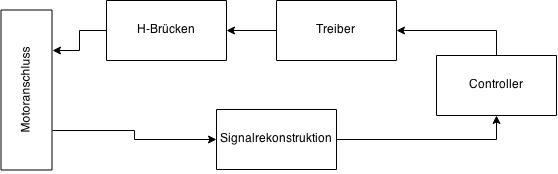
\includegraphics[width=0.8\textwidth,clip,trim=0mm 0mm 0mm 0mm]
   	{\EtPath/Bilder/Blockschaltbild_BLDC.jpg}
   	\centering
   	\caption{Blockschaltbild des BLDC-Boards}
   	\label{abb:BlockschaltbildBLDC}
\end{figure}\\
In der Abbildung \ref{abb:BlockschaltbildBLDCPhoto} ist die Realisierung der Blöcke ersichtlich. 
Dabei ist der erste Kasten der Anschluss des Motors, der zweite die H-Brücken, der dritte der 
Treiber, der vierte die Signalrekonstruktion und der fünfte Teil ist der Controller, auf dem 
die Firmware läuft.
\begin{figure}[h!]
   	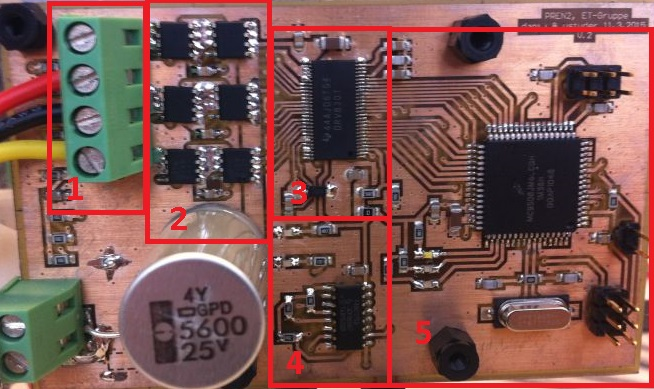
\includegraphics[width=0.8\textwidth,clip,trim=0mm 0mm 0mm 0mm]
   	{\EtPath/Bilder/BLDC-BoardBloecke.jpg}
   	\centering
   	\caption{Blockschaltbild des BLDC-Boards}
   	\label{abb:BlockschaltbildBLDCPhoto}
\end{figure}

\ifSTANDALONE
\subsection{Kommutierung}
\fi
\ifEMBED
\paragraph{Kommutierung}$~~$\vspace{2mm}\\
\fi
Der Motor wird mit drei Halbbrücken kommutiert. Für die Ansteuerung der MOSFET\footnote{metal-oxide-semiconductor field-effect transistor} 
wird ein Predriver DRV8301 von Texas Instruments eingesetzt. Die Halbbrücken 
werden einzeln vom Controller geschalten. Damit nur ein 
PWM\footnote{\textbf{P}ulse \textbf{W}idth \textbf{M}odulation}-Signal erzeugt 
werden muss, werden die Ansteuerleitungen mittels Widerständen mit dem 
PWM-Signal verbunden. Werden die Ansteuerungen vom Controller nicht aktiv 
getrieben, liegt die PWM an. Die Konfiguration der Predrivers erfolgt über SPI. 

\ifSTANDALONE
\subsection{Phasendetektion}
\fi
\ifEMBED
\paragraph{Phasendetektion}$~~$\vspace{2mm}\\
\fi
Die Phasendetektion besteht aus Sternpunktnachbildung, Komparator und 
Synchronisation. Die Sternpunktnachbildung erzeugt einen virtuellen Sternpunkt 
mit Hilfe eines Widerstandsnetzwerkes und eines Tiefpassfilters. Die einzelnen 
Phasenspannungen werden mit diesem virtuellen Sternpunkt verglichen. Mit einem 
Flipflop wird das Signal mit der PWM Synchronisiert. 

\ifSTANDALONE
\subsection{Controller}
\fi
\ifEMBED
\paragraph{Controller}$~~$\vspace{2mm}\\
\fi
Als Controller kommt ein HC9S08JM60 der Firma Freescale zum Einsatz. Der Takt 
wird mittels Quarz mit 12MHz erzeugt. Um den aktuellen Betriebsszustand 
anzuzeigen, stehen drei LED zur Verfügung. 

\ifSTANDALONE
\subsection{Speisung}
\fi
\ifEMBED
\paragraph{Speisung}$~~$\vspace{2mm}\\
\fi
Die Eingangsspannung wird mittels eines optional bestückbaren Filters von 
Murata gefiltert. Der Predriver wird direkt mit dieser gefilterten Speisung 
betrieben. Mit dem im Predriver integrierten Step-Down-Converter wird eine 
Spannung von 3.3\si{\volt} erzeugt. Für Varianten mit hoher Betriebsspannung (>30\si{\volt}) 
wird der Komparator der Phasendetektion über einen diskret aufgebauten 
Spannungsregler mit einer Spannung von 30\si{\volt} versorgt. 


\ifSTANDALONE
\section{Firmware}
\fi
%\ifEMBED
%\subsection{Firmware}
%\fi

\subsection{Übersicht}

\ifSTANDALONE
\subsection{Takt}
\fi
\ifEMBED
\subsubsection{Takt}
\fi
Der Referenztakt wird durch einen Quarz mit einer Frequenz von 
12\si{\mega\hertz} erzeugt.  Dieser Takt dient als Referenztakt für die PLL 
des HS9S08JM60. Dazu wird er durch 8 geteilt um im erlaubten 
Bereich\footnote{Die Frequenz des Eingangssignals der PLL muss im Bereich 1 
\ldots 2\si{\mega\hertz} liegen. \cite[p.  195]{Datasheet:HCS08}} für die PLL 
zu liegen. In der PLL wird der Takt mit 32 multipliziert. Dies ergibt einen 
CPU Takt von 48\si{\mega\hertz}. Da der Bustakt der Hälfte des CPUtakts 
entspricht, weist dieser eine Frequenz von 24\si{\mega\hertz} auf.  Der 
Externe Takt (16\si{\mega\hertz}) wird zusätzlich als externer Referenztakt 
zur Verfügung gestellt und vom RTC verwendet.  (siehe auch Abschnitt 
\ref{sec:rtc} \nameref{sec:rtc})

\ifSTANDALONE
\subsection{RTC}
\fi
\ifEMBED
\subsubsection{RTC}
\fi
\label{sec:rtc}
Um regelmässig abzuarbeitende Aufgaben zu steuern, wird ein entsprechender 
Takt benötigt. Dafür wird der RTC\footnote{\textbf{R}eal \textbf{T}ime 
\textbf{Counter}} verwendet. Dieser verwendet als Takt den externen 
Referenztakt mit einer Frequenz von 16\si{\mega\hertz}. Dieser wird mit dem 
Prescaler auf eine Frequenz von 16\si{\kilo\hertz} geteilt. Über das Modulo 
Register kann eine Periodendauer im Bereich 62.5\si{\micro\second} \ldots 
16\si{\milli\second} eingestellt werden. Es wird zunächst eine Periodendauer 
von 1\si{\milli\second} verwendet. In der ISR\footnote{\textbf{I}nterrupt 
\textbf{S}ervice \textbf{Routine}} wird ein Flag gesetzt, welches in der 
Hauptschlaufe abgefragt wird. 
\begin{table}[h!]
    \begin{zebratabular}{p{0.10\textwidth}p{0.06\textwidth}p{0.25\textwidth}p{0.5\textwidth}}
    \rowcolor{gray} Register & Wert & Beschreibung & Bemerkungen \\
    RTCSC &
        \verb!0x38! &
        RTC Status and Control Register &
        ERCLK, Interrupts enabled, Prescaler = $10^3$ $\to$ T$_{\text{Count}}$ = $\frac{1}{16}$\si{\milli\second} \\
    RTCMOD &
        \verb!0x0F! &
        RTC Modulo Register &
        Modulo = 15 $\to$ T$_{\text{Interrupt}}$ = 1\si{\milli\second} \\
    \end{zebratabular}
    \caption{Registerinitialisierung RTC}
    \label{tab:rtc_init}
\end{table}

\subsection{PWM}
Mit der PWM\footnote{\textbf{P}ulse \textbf{W}idth \textbf{M}odulation} werden 
die Ausgangsstufen angesteuert. Über das Puls - Pausenverhältnis wird die 
Leistung eingestellt. Damit diese Ansteuerung jedoch nicht hörbar wird, muss 
der Motor mit einer PWM Frequenz oberhalb des hörbaren Frequenzbereichs des 
Menschen angesteuert werden. Es wird eine Frequenz von 24\si{\kilo\hertz} 
verwendet.  Für das Erzeugen der PWM wird der Timer TPM2 verwendet. 
\begin{table}[h!]
    \begin{zebratabular}{p{0.10\textwidth}p{0.06\textwidth}p{0.25\textwidth}p{0.5\textwidth}}
    \rowcolor{gray} Register & Wert & Beschreibung & Bemerkungen \\
    TPM2SC &
        \verb!0x08! &
        TPM2 Status and Control Register &
        Overflow interrupt disabled, no Center-aligned PWM, Bus clock as clock 
            source, Prescaler = 1\\
    TPM2CNT &
        \verb!0x____! &
        TPM2 Counter Register &
        No initialisation \\
    TPM2MOD &
        \verb!0x03FF! &
        TPM2 Counter Modulo Register &
        1023 $\to$ $\frac{24\si{\mega\hertz}}{1024} = 23.4375\si{\kilo\hertz}$  \\
    TPM2C0SC &
        \verb!0x28! &
        TPM2 Channel 0 Status and Control Register &
        Interrupt disabled, edge aligned PWM, High-true\\
    TPM2C0V &
        \verb!0x0033! &
        TPM2 Channel 0 Value Register &
        5\si{\percent} \\
    TPM2C1SC &
        \verb!0x24! &
        TPM2 Channel 1 Status and Control Register &
        Interrupt disabled, edge aligned PWM, Low-true\\
    TPM2C1V &
        \verb!0x03CD! &
        TPM2 Channel 1 Value Register &
        5\si{\percent} \\
    \end{zebratabular}
    \caption{Registerinitialisierung TPM2}
    \label{tab:rtc_init}
\end{table}

\ifSTANDALONE
\subsection{Kommutierungsverzögerung / Zeitmessung}
\fi
\ifEMBED
\subsubsection{Kommutierungsverzögerung / Zeitmessung}
\fi
Um den exakten Kommutierungszeitpunkt einstellen zu können, und um die Zeit 
zwischen zwei Kommutierungen zu messen wird ein weiterer Timer benötigt. Dafür 
wird TPM1 verwendet. Als Taktquelle für den Timer wird der Bustakt mit einer 
Frequenz von 24\si{\mega\hertz} verwendet. Dieser wird mit dem maximal möglichen 
Prescaler von 128 geteilt. Dies ergibt eine Frequenz von 187.5\si{\kilo\hertz} 
und eine Auflösung von 5.33\si{\micro\second}. Damit ist eine maximale 
Messdauer von 349.5\si{\milli\second} möglich. 
\begin{table}[h!]
    \begin{zebratabular}{p{0.10\textwidth}p{0.06\textwidth}p{0.25\textwidth}p{0.5\textwidth}}
    \rowcolor{gray} Register & Wert & Beschreibung & Bemerkungen \\
    TPM1SC &
        \verb!0x0F! &
        TPM1 Status and Control Register &
        Overflow interrupt disabled, no Center-aligned PWM, Bus clock as clock 
            source, Prescaler = 128\\
    TPM1CNT &
        \verb!0x____! &
        TPM1 Counter Register &
        No initialisation \\
    TPM1MOD &
        \verb!0x0000! &
        TPM1 Counter Modulo Register &
        Free running \\
    TPM1C0SC &
        \verb!0x50! &
        TPM1 Channel 0 Status and Control Register &
        Interrupt enabled, Output compare \\
    TPM1C0V &
        \verb!0x0000! &
        TPM1 Channel 0 Value Register &
        Used for commutation delay of phase U \\
    TPM1C1SC &
        \verb!0x50! &
        TPM1 Channel 1 Status and Control Register &
        Interrupt enabled, Output compare \\
    TPM1C1V &
        \verb!0x0000! &
        TPM1 Channel 1 Value Register &
        Used for commutation delay of phase V \\
    TPM1C2SC &
        \verb!0x50! &
        TPM1 Channel 2 Status and Control Register &
        Interrupt enabled, Output compare \\
    TPM1C2V &
        \verb!0x0000! &
        TPM1 Channel 2 Value Register &
        Used for commutation delay of phase W \\
    TPM1C3SC &
        \verb!0x44! &
        TPM1 Channel 3 Status and Control Register &
        Interrupt enable, input capture \\
    TPM1C3V &
        \verb!0x0000! &
        TPM1 Channel 3 Value Register &
        Initialized zero, value not used later \\
    TPM1C4SC &
        \verb!0x44! &
        TPM1 Channel 4 Status and Control Register &
        Interrupt enable, input capture \\
    TPM1C4V &
        \verb!0x0000! &
        TPM1 Channel 4 Value Register &
        Initialized zero, value not used later \\
    TPM1C5SC &
        \verb!0x44! &
        TPM1 Channel 5 Status and Control Register &
        Interrupt enable, input capture \\
    TPM1C5V &
        \verb!0x0000! &
        TPM1 Channel 5 Value Register &
        Initialized zero, value not used later \\
    \end{zebratabular}
    \caption{Registerinitialisierung TPM1}
    \label{tab:rtc_init}
\end{table}


\ifSTANDALONE
\subsection{Kommunikation zum Host}
\fi
\ifEMBED
\subsubsection{Kommunikation zum Host}
\fi
Zur Interaktion mit dem BLDC-Board wird die SPI1-Schnittstelle des $\mu C$ verwendet. Dabei
ist das SPI-Interface im 8 Bit Mode mit LSB-First konfiguriert. Zusätzlich zu dieser Schnittstelle
ist eine IRQ-Leitung vorhanden, mit der das BLDC-Board den Host triggern kann, um auf ein Problem 
hinzuweisen. Die Steckerbelegung ist in Tabelle \ref{tab:SPI_stecker} ersichtlich.
\begin{table}[h!]
    \begin{zebratabular}{p{0.10\textwidth}p{0.06\textwidth}p{0.25\textwidth}p{0.5\textwidth}}
    \rowcolor{gray} Register & Wert & Beschreibung & Bemerkungen \\
    SPI1C2 &
        \verb!0x00! &
        SPI Control Register 2 & 
        \\
    SPI1C1 &
        \verb!0x85! &
        SPI Control Register 1 &
        IRQ-Enable aktiviert und LSB-First konfiguriert\\
    \end{zebratabular}
    \caption{Registerinitialisierung SPI1}
    \label{tab:spi1_init}  
\end{table}

\begin{table}[h!]
    \begin{zebratabular}{p{0.10\textwidth}p{0.06\textwidth}}
    \rowcolor{gray} Pin & Name\\
    1 & GND\\
    2 & MISO\\
    3 & CS\\
    4 & MOSI\\
    5 & CLK\\
    6 & IRQ\\
    \end{zebratabular}
    \centering
    \caption{Steckerbelegung der SPI-Schnittstelle}
    \label{tab:SPI_stecker}
\end{table}
Die Kommunikation zwischen BLDC-Board und Host funktioniert über ein Protokoll zur Interaktion. die 
Spezifikation dieses ist in der Tabelle \ref{tab:Spi_Int_Table} ersichtlich. Das obere Nibble des
CMD's enthält den Befehl und das untere Nibble die Anzahl Argumente, die zum CMD gehören.
Wenn das untere Nibble \verb!0xF! ist, wird die Länge der Übertragung im nächsten Byte signalisiert.
\begin{table}[h!]
    \begin{zebratabular}{p{0.12\textwidth}p{0.06\textwidth}p{0.35\textwidth}p{0.4\textwidth}}
    \rowcolor{gray} Name & Wert & Beschreibung & Parameter\\
    Dummy &
        \verb!0x00! & 
        Byte das benötigt wird, um zu clocken für die Übertragung von Argumenten &
        \\
    Start &
        \verb!0x10! & 
        Startet den Motor &
        \\
    Stop &
        \verb!0x20! & 
        Stoppt den Motor &
        \\
    setRPM &
        \verb!0x32! & 
        16 Bit Zahl um die Drehzahl einzustellen & 
        1. Byte = High-Byte\newline 
        2. Byte = Low-Byte\\
    setVoltage &
        \verb!0x42! & 
        $U_{GS}$ der FET's. & 1. Byte = Spannungswert-High-Byte\newline 
                              2. Byte = Spannungswert-Low-Byte\\
    setCurrent &
        \verb!0x51! & 
        Wert der Strombegrenzung. Der Stromwert ergibt sich nach der Formel $Current = Wert \cdot 10$ &
        $Registerwert = \frac{Sollwert\; in \;[mA]}{10} $\\
    getStatus &
        \verb!0x64! & 
        Gibt der Board-Status zurück &
        1. Byte = Motor-Status\newline
        2. Byte = Fehler-Code\newline
        3. Byte = RPM-High-Byte\newline
        4. Byte = RPM-Low-Byte\\
    areYouAlive &
        \verb!0x71! & 
        Damit kann die Kommunikation und das BLDC-Board testen &
        Das BLDC-Board gibt \verb!0x55! zurück\\
    setPwm &
        \verb!0x81! & 
        Damit kann die PWM des Motors eingestllt werden &
        PWM-Wert im Bereich 1-100 \% \\
    startMessung Param &
        \verb!0xC3! & 
        Messung parametrisiert starten &
        1. Byte = Pulsdauer\newline
        2. Byte = RPM-High-Byte\newline
        3. Byte = RPM-Low-Byte\\
    startMessung &
        \verb!0xD0! & 
        Messung mit einem Schritt starten &
        \\
    getMessung &
        \verb!0xEF! & 
        gibt die gespeicherte Messung zurück &
        1. Byte = Länge\newline
        2. - n. Byte = Daten der Messung\\
    \end{zebratabular}
    \caption{Kommunikationsprotokoll}
    \label{tab:Spi_Int_Table}
\end{table}



\begin{table}[h!]
    \begin{zebratabular}{p{0.07\textwidth}p{0.07\textwidth}p{0.07\textwidth}p{0.07\textwidth}p{0.07\textwidth}p{0.07\textwidth}p{0.07\textwidth}p{0.07\textwidth}}
    \rowcolor{gray} \multicolumn{8}{|c|}{Mögliche Werte als Argument für setVoltage }\\
    $60 mV$   & $68 mV$   & $76 mV$   & $86 mV$   & $97 mV$   & $109 mV$  & $123 mV$  & $138 mV$  \\
    $155 mV$  & $175 mV$  & $197 mV$  & $222 mV$  & $250 mV$  & $282 mV$  & $317 mV$  & $358 mV$  \\
    $403 mV$  & $454 mV$  & $511 mV$  & $576 mV$  & $648 mV$  & $730 mV$  & $822 mV$  & $926 mV$  \\
    $1046 mV$ & $1175 mV$ & $1324 mV$ & $1491 mV$ & $1679 mV$ & $1892 mV$ & $2131 mV$ & $2400 mV$ \\
    \end{zebratabular}
        \centering
    \caption{Gültige Wert als Argument für setVoltage}
\end{table}


